\documentclass[12pt,oneside,letterpaper,english]{article}
\usepackage[T1]{fontenc}
\usepackage[latin1]{inputenc}
\usepackage[margin=2.25cm,headheight=26pt,includeheadfoot]{geometry}
\usepackage[english]{babel}
\usepackage{listings}
\usepackage{color}
\usepackage{titlesec}
\usepackage{titling}
\usepackage[framed, numbered]{matlab-prettifier}
\usepackage{changepage}
\usepackage{amsmath}
\usepackage{hyperref}
\usepackage{enumitem}
\usepackage{graphicx}
\usepackage{fancyhdr}
\usepackage{lastpage}
\usepackage{caption}
\usepackage{tocloft}
\usepackage{setspace}
\usepackage{multirow}
\usepackage{titling}
\usepackage{float}
\usepackage{comment}
\usepackage{booktabs}
\usepackage{indentfirst}
\usepackage{lscape}
\usepackage{booktabs,caption}
\usepackage[flushleft]{threeparttable}
\usepackage[english]{nomencl}
\usepackage{xcolor}
\usepackage{lipsum}
\usepackage{datetime2}
\usepackage{natbib}


\bibliographystyle{plainnat} 



% --- set footer and header ---
\pagestyle{fancy}
\fancyhf{}

\setlength{\parindent}{2em}
\title{Multiple spliced alignment : a consistency based Approach} % to reference as \title, dont use \maketitle
\makeatletter\let\Title\@title\makeatother



\lstset{language=Matlab,
style=Matlab-editor,
basicstyle=\normalsize\mlttfamily,
numbers=left,
numberstyle={\scriptsize\color{black}},	% size of the numbers
numbersep=0.5cm											
}

\newlist{steps}{enumerate}{1}
\setlist[steps, 1]{leftmargin=1.5cm,label = Step \arabic*:}
\renewcommand{\headrulewidth}{1pt}
\renewcommand{\footrulewidth}{1pt}
\renewcommand{\rmdefault}{ptm}

%\lhead{\Title}
\rhead{\nouppercase{\rightmark}}
\lhead{\Title}
\rfoot{
\includegraphics[height=0.7cm]{figures/241208906_10159878130857049_3729368319539169165_n.png}} % right header logo
\setlength\headheight{16pt}
\setlength{\footskip}{50pt}
\lhead{\Title} %rightH title
\cfoot{\thepage}

% --- End of page settings ---



\begin{document}
\pagenumbering{roman} 

\begin{titlepage}
\begin{center}
\vspace{2cm}
%\textsc{Oregon State University}\\[1.5cm]

\includegraphics[width=0.4\textwidth]{figures/udeslog.png}~\\[1cm]
\vspace{2cm}

% Title
\hrule
\vspace{.5cm}
{ \huge \bfseries Multiple Spliced Alignment : \\ A Consistency Based Approach} % title of the report
\vspace{.5cm}

\hrule
\vspace{1.5cm}

\textsc{\textbf{Author}}\\
\vspace{.5cm}
\centering

% add your name here
Chakirou ALABANI (Group H)\\


\vspace{8cm}

% \centering \today \\ % see latexmkrc for time zone change
\centering BIN702 - Autumn 2024 \\ 
\centering Nadia Tahiri
\end{center}
\end{titlepage}

\newpage
\doublespacing
%\addcontentsline{toc}{section}{Table of Contents}
\renewcommand{\baselinestretch}{1}\normalsize
\tableofcontents
\renewcommand{\baselinestretch}{1}\normalsize
%\singlespacing
\thispagestyle{fancy} % force page style

\newpage
\pagenumbering{arabic} 
\fancyfoot[C]{Page \thepage\ of \pageref{EndOfText}}

\section{Project description}
Alternative splicing is now recognized as a fundamental process in eukaryotic organisms, enabling a single 
gene to generate multiple distinct transcripts. This mechanism affects the majority of human genes 
(\textit{\citep{harrow2006gencode, tress2007implications, kim2008alternative, wang2008alternative, chen2009mechanisms}}) 
and is widely pervasive, playing a crucial role in enhancing the diversity of
the proteome. 
Recent genome-wide studies indicate that 40--60\% of human genes have alternatively spliced forms (\textit{\citep{modrek2002genomic}}). 
This extensive occurrence underscores the need to investigate the evolutionary and conservation patterns of transcript sets, as these 
insights are essential for a deeper understanding of the mechanisms that influence gene evolution.


Understanding the evolution of sets of alternative transcripts is a challenging task and requires automated methods and tools to compare
sets of alternative transcripts from homologous genes. 
Alternative transcripts from homologous genes have traditionally been compared using pairwise spliced 
alignments (PSpAs). A PSpA aligns either a spliced RNA sequence or its DNA equivalent, the coding DNA 
sequence (CDS), with an unspliced DNA sequence. This approach helps identify homologous or corresponding 
exons between sequences, providing crucial insights for genome annotation and gene prediction
(\textit{\citep{stanke2006augustus, dunne2018omgene}}). Various methods have been developed to tackle 
different versions of the PSpA problem, which involves finding the best PSpA between two sequences based 
on a specific optimization function (see \textit{\citep{jammali2019splicedfamalign}}). However, PSpA is limited to 
comparing only two sequences at a time, making it unsuitable for examining the evolution of alternative splicing. 
This restriction also renders it ineffective for analyzing large databases, where multiple sequence comparisons are 
essential.

A logical extension of pairwise spliced alignment (PSpA) for studying the evolution of alternative spliced RNA sets is 
multiple spliced alignment (MSpA). This approach aligns a collection of spliced RNA sequences with their corresponding 
unspliced genomic sequences, allowing for detailed analysis of splicing and exon structures within the gene sequences. 
Unlike traditional multiple sequence alignment (MSA), which focuses solely on sequence similarity, MSpA incorporates the 
splicing and exonic architectures of the input genes. Just as MSA has greatly advanced our understanding of sequence 
evolution, MSpA is anticipated to reveal new insights into the evolution of alternative splicing and the relationships 
among alternative spliced RNA sets.

The MSpA framework also has practical applications for genome annotation by facilitating the identification of exons homologous 
to those in well-characterized species, thereby aiding in the prediction of conserved isoforms in newly annotated genomes.

In the current state of art, there are a few methods available for coomputong MSpAs, with SplicedFamAlignMulti (SFAM) being a 
leading approach (\textit{\citep{jammali2022pairwise}}). SFAM include three extensions : SFAM\_mblock, SFAM\_tcoffee\_p, 
and SFAM\_tcoffee\_m, each providing tailored functionalities for different alignment scenarios. A summary of SFAM methods 
mechanisms is shown in Figure~\ref{fig:spfam-ov}.

\begin{figure}
    \centering
    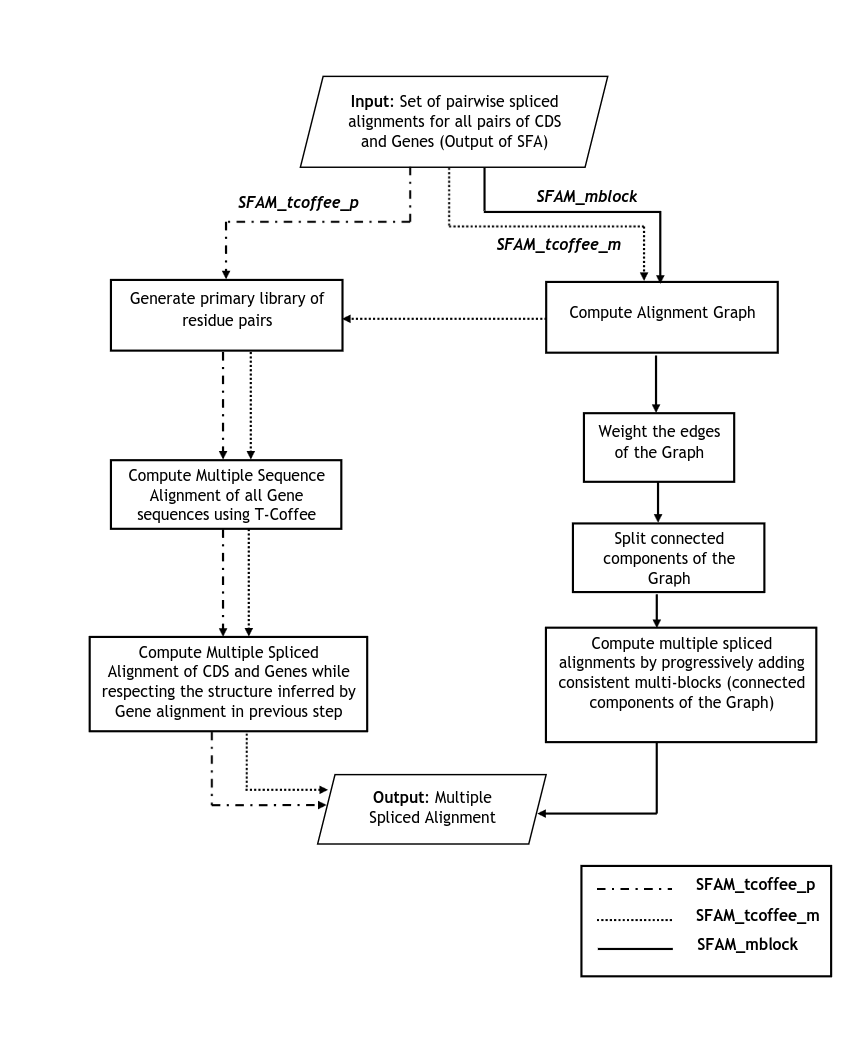
\includegraphics[width=0.3\linewidth]{figures/overview_spFam_methods.png}
    \caption{overview SFAM methods}
    \label{fig:spfam-ov}
\end{figure}

In this report, we present SplicedFamAlignMultiCBA (SFAM\_CBA), a greedy heuristic method developed to merge all 
pairwise spliced alignments (PSpAs) of known coding sequences (CDSs) and gene sequences within a gene family into a 
multiple spliced alignment (MSpA).

 

\section{Materials and methods}
\subsection{Characterization of the MSpA Problem}
\subsubsection{Pairwise Spliced Alignment (PSpA)}
A Pairwise Spliced Alignment (PSpA) refers to the alignment of a Coding Sequence (CDS) with a gene sequence while accounting for the splicing structure. This alignment aims to identify homologous exon sequences and is formulated as a chain of blocks, where each block corresponds to pairwise alignments of segments from both the CDS and gene. 

The significance of PSpA lies in its ability to highlight macroscopic alignments at the splicing level (exon intron structure) rather than at the nucleotide level, emphasizing differences in splicing trends and exon usage across gene families.

\textbf{Definition:} A PSpA consists of blocks, which are conserved segments where both the CDS and gene are included in the alignment. If a CDS is aligned with a gene in a block, it is termed a \textit{conserved block}. Conversely, if only the CDS is included, it is referred to as a \textit{deleted block}.

\subsubsection{Multiple Spliced Alignment (MSpA)}

An MSpA extends the concept of PSpA to include multiple CDSs and gene sequences, facilitating the identification of homologous exons across a broader set of sequences. 

\textbf{Definition:} An MSpA of a set of CDSs \( C \) and genes \( G \) is represented as a chain of multiblocks \( A = \{A[1], \ldots, A[n]\} \). Each multiblock \( A[i] \) includes a key set \( \text{key}(A[i]) \), which is a subset of \( C \cup G \), mapping each sequence to its respective start and end locations \( (s^x_i, e^x_i) \).

The MSpA must satisfy several conditions:
\begin{itemize}
    \item Each multiblock must contain at least one element.
    \item Segments from the same sequence must not overlap across multiblocks.
    \item The segments induced by the MSpA must fully cover the original CDSs.
    \item Segments from aligned genes must be consistent within the same multiblock.
\end{itemize}

\subsubsection{Multiple spliced alignment problem }
\textbf{Input:} A set of CDSs \( C \); a set of genes \( G \), a set of PSpAs \( X = \{ X_{c,g} \mid (c, g) \in C \times G \} \) for all pairs in \( C \times G \).

\textbf{Output:} An MSpA \( A \) of \( C \) on \( G \) that maximizes the sum of the scores of induced PSpAs: \[
\sum_{(c,g) \in C \times G} S(A_{c,g})\] (\textit{\cite{jammali2022pairwise}}).

Several methods are available for computing PSpAs between a gene and a CDS (\textit{\cite{jammali2019splicedfamalign}}).

\subsection{The SFAM-CBA algorithm}
We now present our algorithm for constructing an MSpA for a set of CDSs \( C \) and a set of genes \( G \),
given a set of PSpAs \( X = \{ X_{c,g} \mid (c, g) \in C \times G \} \) for all pairs in \( C \times G \) 
(the MSAPproblem). MSA methods commonly employ greedy heuristics, with the progressive alignment 
strategy (\textit{\cite{feng1987progressive}}) being one of the most widely used approaches.
Distinctively, our method incorporates both the consistency approach and the triplet approach outlined \
in \textit{\cite{t_coffee_alignment}} for pairwise scoring. The consistency-based strategy evaluates how well the alignment of two 
residues or segments in a given pairwise alignment is supported by other precomputed pairwise alignments. Applying this consistency-based 
approach within a progressive alignment allows for the integration of information from all pairwise alignments at each step, 
helping to overcome the typical limitations associated with progressive alignment.

\subsubsection{Boundaries refinement}

Boundary refinement is a crucial step in the consistency based approch for MSpA, aiming to handle overlapping segment matches effectively. 
The refinement algorithm extends the principles established by \textit{Halpern et al. (2002)}, ensuring that all parts of the original segment 
matches can be utilized. 

As described in \textit{\cite{feng1987progressive}}, let \( M = \{M_0, M_1, \ldots, M_{m-1}\} \) represent the set of segment matches, where each match \( M_k = (S_i^{uv}, S_j^{xy}) \) 
consists of segments \( S_i^{uv} \) from sequence \( S_i \) and \( S_j^{xy} \) from sequence \( S_j \). The goal is to refine these segment 
matches into a set of submatches \( M^* = \{M_0^*, M_1^*, \ldots, M_{m'-1}^*\} \) that cover the original matches.

In this context, the refinement process involves ensuring that the set of submatches \( M^* \) satisfies the conditions of tiling the 
original matches:
\[
[u, v - 1] = \bigcup_{M_k' \in M'_*} [u', v' - 1] \quad \text{and} \quad [x, y - 1] = \bigcup_{M_k' \in M'_*} [x', y' - 1].
\]
This ensures that each original match is fully covered by the refined submatches in \( M^* \). 

A resolved set of matches, denoted as \( R \), is desired, where all segments are either disjoint or identical. In such a set, any \( (S_i^{uv}, S_j^{xy}) \in R \) satisfies:
\[
[u, v] \cap \text{supp}_S^i(R) = \{u, v\} \quad \text{and} \quad [x, y] \cap \text{supp}_S^j(R) = \{x, y\}.
\]
The algorithm proceeds to process segment matches sequentially, building a node set \( V_i \) for each sequence \( S_i \), initialized to the support set of the segments. By recursively identifying boundary positions and ensuring necessary cuts are made, the algorithm guarantees a minimum cardinality refinement without introducing superfluous cuts.

% 

\subsubsection{Pairwise Spliced Alignment (PSpA)}

A Pairwise Spliced Alignment (PSpA) refers to the alignment of a Coding Sequence (CDS) with a gene sequence while accounting for the splicing structure. This alignment aims to identify homologous exon sequences and is formulated as a chain of blocks, where each block corresponds to pairwise alignments of segments from both the CDS and gene. 

The significance of PSpA lies in its ability to highlight macroscopic alignments at the splicing level (exon–intron structure) rather than at the nucleotide level, emphasizing differences in splicing trends and exon usage across gene families.

\textbf{Definition:} A PSpA consists of blocks, which are conserved segments where both the CDS and gene are included in the alignment. If a CDS is aligned with a gene in a block, it is termed a \textit{conserved block}. Conversely, if only the CDS is included, it is referred to as a \textit{deleted block}.

\subsubsection{Multiple Spliced Alignment (MSpA)}

An MSpA extends the concept of PSpA to include multiple CDSs and gene sequences, facilitating the identification of homologous exons across a broader set of sequences. 

\textbf{Definition:} An MSpA of a set of CDSs \( C \) and genes \( G \) is represented as a chain of multiblocks \( A = \{A[1], \ldots, A[n]\} \). Each multiblock \( A[i] \) includes a key set \( \text{key}(A[i]) \), which is a subset of \( C \cup G \), mapping each sequence to its respective start and end locations \( (s^x_i, e^x_i) \).

The MSpA must satisfy several conditions:
\begin{itemize}
    \item Each multiblock must contain at least one element.
    \item Segments from the same sequence must not overlap across multiblocks.
    \item The segments induced by the MSpA must fully cover the original CDSs.
    \item Segments from aligned genes must be consistent within the same multiblock.
\end{itemize} 

\subsubsection{Computation of pairwise scores}

The computation of pairwise scores of the set of PSpAs \( X = \{ X_{c,g} \mid (c, g) \in C \times G \} \) is vital for quantifying the similarity between aligned segments of 
sequences. This process relies on the refined segment matches obtained in the previous step. 

Given a set of refined matches \( M^* \), the pairwise score \( S_{ij} \) between sequences \( S_i \) 
and \( S_j \) can be calculated as follows:
\[
S_{ij} = \sum_{k} \text{idty}(M_k^{*}),
\]
where \( \text{idty}(M_k^{*}) \) represents the identity score of the match \( M_k^{*} \) that covers the 
segment \( (S_i^{uv}, S_j^{xy}) \). The identity score can be derived from established scoring matrices 
adjusted for the context of the segments being compared.

To incorporate information from multiple sequences, a weight system can be applied, similar to the one 
discussed by Notredame et al. (1998). By considering intermediate sequences that support the alignment, 
the weights associated with each residue pair are aggregated, enhancing the reliability of the pairwise 
scores. 

The overall weight \( W \) for a pair of aligned residues is computed by examining triplets of sequences 
and accumulating scores based on their alignments. The final weight reflects both the similarity of the 
sequences and their consistency across the dataset, facilitating a more robust alignment process.

\subsubsection{MSpA Computation}

The final stage involves the computation of the multiple sequence alignment (MSA) itself. This process is 
executed through a recursive algorithm that utilizes the refined pairwise scores obtained in the previous 
steps. The goal is to construct an alignment that maximizes the overall score while adhering to the 
constraints imposed by the segment matches.

Let \( T \) represent the phylogenetic tree that organizes the sequences based on their evolutionary 
relationships. The MSpA can be computed recursively as follows:
\[
C(T_i) = \text{Align}(C(T_{\text{left}}), C(T_{\text{right}}), S),
\]
where \( C(T_i) \) is the column list of aligned sequences at node \( T_i \) and \( S \) is the pairwise score matrix derived from the previous computations.

Each internal node of the tree represents an alignment of its child nodes. The alignment function 
\( \text{Align} \) combines the column lists from the left and right child nodes, optimizing the alignment 
based on the accumulated pairwise scores:
\[
\text{Align}(C(T_{\text{left}}), C(T_{\text{right}}), S) = \max_{\text{alignment}} \sum_{\text{pairs}} 
S_{ij},
\]
where the sum is taken over all pairs of aligned segments, and the maximum is computed over all possible 
alignments.

This recursive approach allows the algorithm to build the MSpA incrementally, ensuring that the final 
alignment is optimal with respect to the defined scoring system. The use of a refined weight system 
ensures that the alignment reflects not only the local similarities but also the global relationships 
among all sequences, thereby enhancing the quality and reliability of the MSpA.



\subsection{Experimental setup}
A comprehensive and detailed pseudocode of each step in the algorithm is provided in the appendix. 
The implementation of the algorithm, along with the data used, is available on GitHub at

\label{EndOfText}

\newpage
\pagenumbering{Roman} 
\addcontentsline{toc}{section}{List of Figures}
\fancyfoot[C]{Page \thepage\ of \pageref{endOfDoc}}
\listoffigures
\thispagestyle{fancy}

\newpage
\addcontentsline{toc}{section}{List of Tables}
\listoftables
\thispagestyle{fancy}

\newpage
\addcontentsline{toc}{section}{References}
% \bibliography{} 
\bibliography{document}
% \bibliographystyle{plainnat}

\newpage
\section{Appendix} \label{ch6}

\label{endOfDoc}
\end{document}
